%%% CSE 4316 Individual Sprint Report - WORKED EXAMPLE (Computer Vision / ML)
\documentclass{article}
\usepackage{siunitx}\usepackage{graphicx}\usepackage{amsmath}
\setlength\parindent{0pt}
\usepackage[letterpaper, portrait, margin=1in]{geometry}
\title{Sprint 2 Report \\ CSE 4316}
\author{Ada Lovelace}
\date{October 20th, 2026}
\begin{document}
\maketitle
\begin{center}
\begin{tabular}{l r}
Sprint start date: & October 6th, 2026 \\
Sprint end date: & October 20th, 2026 \\
Project title: & DigitDesk Handwritten Form Digitization Service \\
Team name: & Team Perceptron \\
Partners: 	& Alan Turing \\
			& Grace Hopper \\
			& John Von Neumann \\
        	& Charles Babbage \\
Instructor: & Christopher D. McMurrough
\end{tabular}
\end{center}

\section{Sprint Goal}
Establish a digit-recognition baseline on public MNIST data and a reproducible
training/evaluation harness, ahead of adapting to real sponsor forms.

\section{Sprint Backlog}
Planned tasks (hours). \\
\begin{tabular}{| p{4in} | >{\centering\arraybackslash} p{1in} | >{\centering\arraybackslash} p{1in} |}
\hline
\textbf{Task description} & \textbf{Estimated work} & \textbf{Actual work} \\ \hline
Load MNIST train/test and build data loaders & 3.0 & 3.0 \\ \hline
Implement CNN classifier (PyTorch) & 5.0 & 4.5 \\ \hline
Training + evaluation harness (reproducible) & 5.0 & 6.0 \\ \hline
Confidence calibration (temperature scaling) & 4.0 & 4.5 \\ \hline
Model versioning + dataset hashing (MS-01) & 3.0 & 3.0 \\ \hline
Draft field-segmentation approach & 4.0 & 4.0 \\ \hline
\textbf{TOTAL} & \textbf{24.0}  & \textbf{25.0} \\ \hline
\end{tabular}

\pagebreak

\section{Individual Time Expenditures}
Tasks performed by the individual (hours). \\
\begin{tabular}{| p{4in} | >{\centering\arraybackslash} p{1in} | >{\centering\arraybackslash} p{1in} |}
\hline
\textbf{Task Description} & \textbf{Actual work} & \textbf{Percent complete} \\ \hline
Implement CNN classifier (PyTorch) & 4.5 & 100\% \\ \hline
Training + evaluation harness & 6.0 & 100\% \\ \hline
Confidence calibration & 4.5 & 90\% \\ \hline
\textbf{TOTAL} & \textbf{15.0}  & \textbf{-} \\ \hline
\end{tabular}

\section{Team Burndown Chart}
Ideal and actual daily team effort are shown below.
\begin{figure}[h]\begin{center}
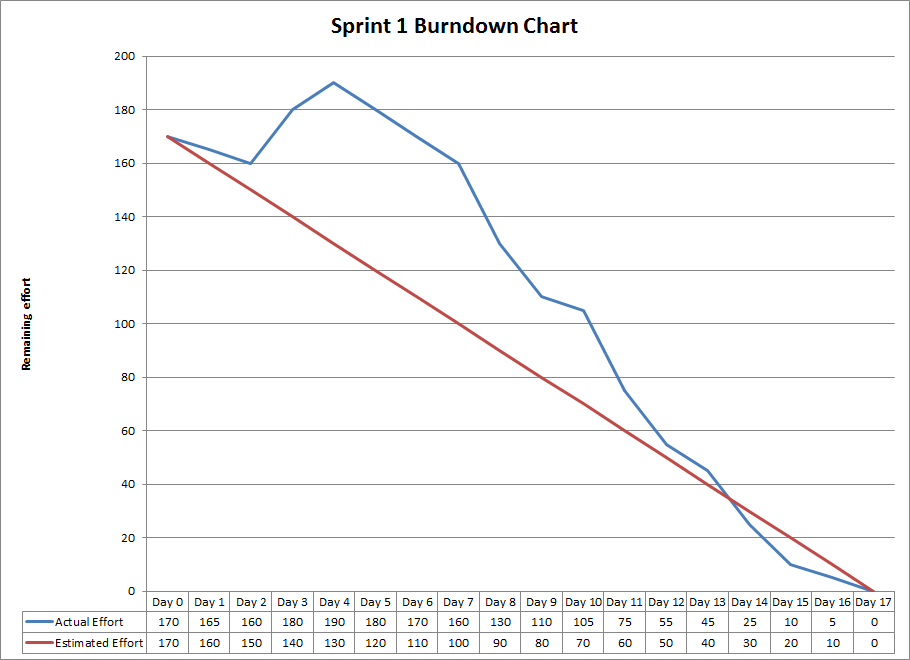
\includegraphics[width=1.0\textwidth]{images/burndown}
\end{center}\end{figure}

\pagebreak

\section{Individual Retrospective}
Actions to \textbf{start} doing (top 3)
\begin{itemize}
\item Fix the evaluation metric and validation split before any tuning.
\item Log every run's model version and dataset hash automatically.
\item Reserve time for the MNIST-to-real domain gap early.
\end{itemize}
Actions to \textbf{stop} doing (top 3)
\begin{itemize}
\item Reporting only top-line accuracy without calibration/error analysis.
\item Training in ad-hoc notebooks that are not re-runnable.
\item Assuming MNIST accuracy will transfer to real forms.
\end{itemize}
Actions to \textbf{continue} doing (top 3)
\begin{itemize}
\item Keeping the model behind a stable, replaceable interface (QA-01).
\item Pairing with John on the segmentation interface contract.
\item Short daily blocker syncs.
\end{itemize}

\section{Peer Review}
Candid individual assessment; not shared. Each item graded 1--5. \\
Evaluation items:
\begin{itemize}
\item \textbf{Participation} - present and contributing?
\item \textbf{Communication} - timely, effective updates?
\item \textbf{Work quality} - claimed tasks; met objectives; added value?
\item \textbf{Professionalism} - professional and collaborative?
\item \textbf{Overall} - overall value this period.
\end{itemize}
\begin{tabular}{| p{1.5in} | >{\centering\arraybackslash} p{1.in} | >{\centering\arraybackslash} p{1.1in} | >{\centering\arraybackslash} p{1.1in}| >{\centering\arraybackslash} p{0.5in}| >{\centering\arraybackslash} p{.5in} |}
\hline
\textbf{Team member name} & \textbf{Participation} & \textbf{Communication} & \textbf{Work quality} & \textbf{Professionalism} & \textbf{Overall} \\ \hline
Ada Lovelace & 5 & 5 & 5 & 5 & 5\\ \hline
Alan Turing & 5 & 5 & 5 & 5 & 5\\ \hline
Grace Hopper & 5 & 4 & 4 & 5 & 4\\ \hline
John Von Neumann & 5 & 4 & 5 & 5 & 5\\ \hline
Charles Babbage & 4 & 4 & 4 & 4 & 4\\ \hline
\end{tabular}
\end{document}
